\section{An ADF Use Case }\label{sec:usecase}
An apparently simple data flow between environments can in fact be complex depending on the nature of the data and the environment(s), the intended data use and the responsibilities of the data situation's stakeholders. When data moves between environments (called a \textit{dynamic data situation} in ADF parlance), each environment produces a different risk profile, depending upon how the data interacts with the the four defining features (other data, governance, infrastructure and agents). To illustrate this, in the next sub-section we will briefly describe an example use case for the ADF. This example is drawn from \cite{elliot2020anonymisation} and is an idealization of a common data situation; the sharing of data held by a national statistics agency with a research data service. Please refer to Figure \ref{fig1} for a visualization. 
\begin{figure}
%\centering
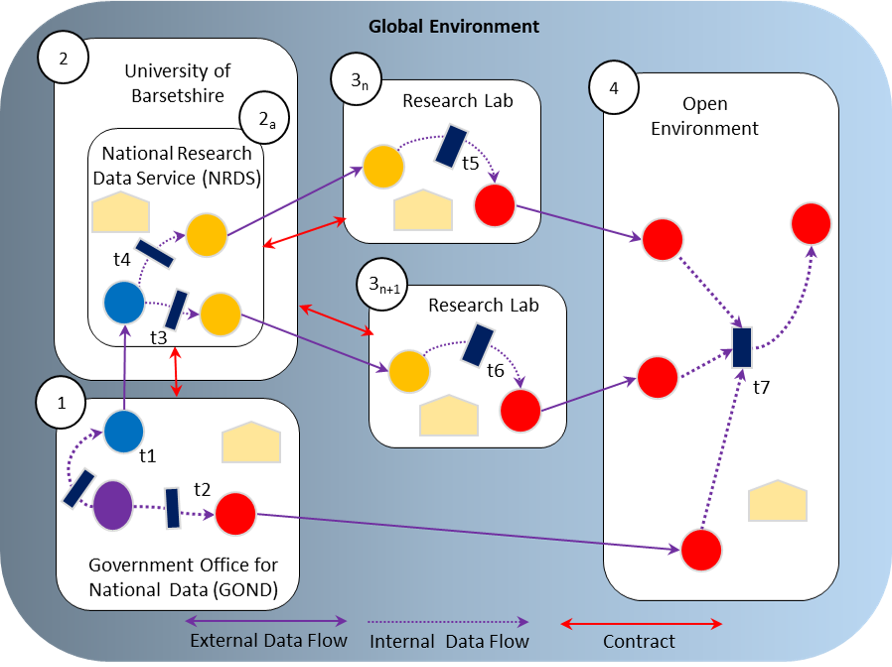
\includegraphics[width=\linewidth]{Picture1a.png}
\caption{A use case of data flows between and within multiple data environments. The red arrows indicate contractual agreements. The blue lines indicate data flow. Data environments are indicated by rounded rectangles, while data (circles), agents (pentagons) and activities (rectangles) are shown within their respective data environments. A circle represents a piece of data, a rectangle represent a process and a pentagon represents a user (in the data environment). The time for processing and sharing of data in the environments are labelled from \begin {math}t_1 \end{math} to \begin {math}t_7\end{math}.} \label{fig1}
\end{figure}
\begin{itemize}
\item Imagine that the Government Office for National Data (GOND) collects many types of national level datasets. For example, national census data, public healthcare data, birth-death related data, pupil data from schools, traffic data from the smart cities sensors, etc.
\item Part of GOND's remit is to make available some of that data for secondary research use. In service of this it shares versions of the national datasets that it holds with the National Research Data Service (NRDS).  
\item GOND also releases highly aggregated data into the public domain (by definition an open environment). 
\item The NRDS is part of University of Barsetshire. The NRDS's role is to acquire data from data holders, including GOND, under contract and then allow (and manage) access to those data under controlled conditions by researchers from research laboratories across the country.
\item The researchers carry out data analysis on GOND's data and then publish papers reporting on this analysis in the public domain. 
\item This data flow involves various loci of responsibility and control over the data sharing in and from the different environments.
\begin{itemize}
\item GOND has indirect responsibility and strategic control over the data release into the open environment (in the form of analytical output within publications). GOND  also has direct responsibility and control over the direct data released from its own environment into the public domain (in the form of aggregate statistics). 
\item NRDS's responsibility and control are different from GOND's, NRDS has direct and operational control over the data release from the output of publications.\footnote{See 
\end{itemize}
\end{itemize}

The sketch diagram of this use case is shown in Figure \ref{fig1}. Four focal data environments are part of global data environment. GOND, the University of Barestshire, and NRDS are represented as data environments 1, 2, and \begin{math}2_{a}\end{math}  respectively. The researchers and open environment are labelled with data environments \begin{math} 3_{n} \end{math} to \begin{math}3_{n+1} \end{math} and 4 respectively. As shown in Figure \ref{fig1}:
\begin{enumerate}
    \item Data starts in a GOND (1) data environment. At $t_1$, it is processed to make it compliant for sharing with (2), according to contractual obligations. At $t_2$, it is processed in a slightly different way to release publically (4).
    \item The data that is shared from GOND to the NRDS (2a), is similarly subjected to additional processing so that it can be shared with various research labs ($3_n,3_{n+1},....$).
    \item Each research lab analyzes the data according to their particular needs and research questions. The research labs wish to produce publications and research datasets for public consumption (4).
    \item One of the major goals of the ADF is to identify when data released by different organizations, that has been derived from the same original data, do not inadvertently disclose information.
\end{enumerate}


\subsection{ADF Requirements (using the GOND-NRDS use case)}
In order to understand the process of anonymisation decision-making in the GOND-NRDS use case a set of requirements have been identified. Based on these requirements, a data environment formalism will be created using W3C PROV data model (PROV-DM). PROV-DM is the conceptual data model and core part of W3C PROV that defines each term used to represent provenance information \cite{moreau2015rationale}.
The GOND-NRDS use case representation (i.e provenance graph) should be able to capture:

A specification of the requirements for representing data environments for the purposes of the ADF illustrated using the GOND-NRDS data situation is shown in table \ref{tab1}.

\begin{table}[!htbp]
 \setlength{\tabcolsep}{5pt}
\caption{Data environment representation requirements for GOND-NRDS use case.\label{tab1}}

%\bigskip
\centering
\begin{sideways}

\begin{tabular}{>{\raggedright\arraybackslash} p{0.2\linewidth} p{0.6\linewidth} p{0.75\linewidth}  }
\hline
\toprule
%\rowcolor{Gray}
\textbf{Requirement}  &  \textbf{Description}  &  \textbf{Example from the GOND-NRDS data situation} \\
%\hline
 \midrule
 \renewcommand{\arraystretch}{1}
Data Environment Construct &
The data environment construct defines a boundary state around data.  data controller, data processor,  data users,  data sharing, data situation, etc. 
%Data environment construct also defines the locus of control and locus of responsibility.
& GOND and NRDS are two closed data environments with different data and events.  \\
\midrule
Data Environments within Data Environments &
Sometimes an environment may contain other environments along with users, data, and processes. And data flows in the same organisation's sub units for processing, auditing, etc. & The NRDS data environment is contained within  the Barestshire university data environment and is an example of environments within environments. \\
\midrule
Attaching Attributes to Data Environments& 
For ADF to determine appropriate disclosure practices,  the purpose of data collection and type of data environment and any constraints and features (infrastructure and governance) of the data environment are attributes of the Data Environment.  &  GOND collects data from its partners for use and onward sharing because of legal obligations. The processing occurs in a restricted access data environment. On the other hand, the data shared through publication in the open environment is not restricted. \\   
\midrule
Relationships between Data Environments &
This describes the possible  relationship from data environment to another data environment & Within the NRDS, a Research Lab may have a specialized, secure processing environment which is owned and maintained by NRDS, but hosted for and used by the Research Lab. This is an example of a data environment with more complex relationships between data environment constructs than containment.\\
\midrule
Annotation to relational constructs & In order to reason over data environment interactions, controllers, processers, subjects, users, etc. it is important to allow the attachment of semantic meaning to the relationships among the constructs &  NRDS receive data from GOND and locally store it for onward to researcher. While in PROV  this can be labeled with \textit{prov:use} and \textit{prov:generated}. It doesn't represent the all of the required information needed by ADF to inform disclosure decisions. \\

Representation of agents, data and processes within a Data Environment & Agents include data controller, data processor, data users and data subjects. Data includes datasets, reports, etc. Processes include data extractions, sharing, storing, etc. &
  As GOND  and NRDS is a type of organisation data controller and processor. GOND is data controller with direct responsibility of his environment and indirect responsibility for NRDS environment. GOND is also a data processor, it generate datasets for NRDS and for an open environment. \\
\midrule
% \midrule
Contracts & 
An agreement or conditions to share, exchange and use data between the environments   &  GOND share data with NRDS based on the  contract between them. \\

\midrule

Access and control (Direct and Indirect)  &
A record of the existing access and control mechanisms over the data and services &  GOND has a data dissemination service/function that can be accessed/used by NRDS (based on some contract or data sharing agreements. GOND has also indirect control over the data release from the NRDS environment.  \\
\bottomrule   
\end{tabular}
\end{sideways}
    \end{table}


